\documentclass[a4paper,12pt]{article}
\usepackage[utf8]{inputenc}% input encoding
\usepackage[T1]{fontenc}% output encoding
\usepackage{lmodern}% fixes czech letters
\usepackage{textcomp}% right arrow, half
\usepackage[none]{hyphenat}% prevent hyphenation
\usepackage[bookmarks,unicode=true]{hyperref}% enable unicode for bookmarks
\usepackage{graphicx}% images
\usepackage[normalem]{ulem}
\usepackage{longtable}
\usepackage{multirow}
\usepackage{array}

% centered table cell "p"
\newcolumntype{P}[1]{>{\centering\arraybackslash}p{#1}}

\setcounter{secnumdepth}{5}% deeper heading numbering
% Word-like margins
\addtolength{\oddsidemargin}{-2cm}
\addtolength{\evensidemargin}{-2cm}
\addtolength{\textwidth}{4cm}
\addtolength{\topmargin}{-2cm}
\addtolength{\textheight}{4cm}

\providecommand{\tightlist}{%
\setlength{\itemsep}{0pt}\setlength{\parskip}{0pt}}

\title{Technické vybavení}
\author{}
\date{}

\begin{document}
\maketitle

\section{Procesory}

\begin{itemize}
\tightlist
\item instrukce = pokyn k vykonání nějaké činnosti
\item instrukční sada = strojový kód
\item překladače: kompilátory, interpretery
\item instrukce: aritmetické, logické, řídící
\item jádro procesoru: ALU, registry, řadič
\item řadič řídí pořadí instrukcí, dostává stavová hlášení
\item zjednodušené blokové schéma procesoru:
\item[] 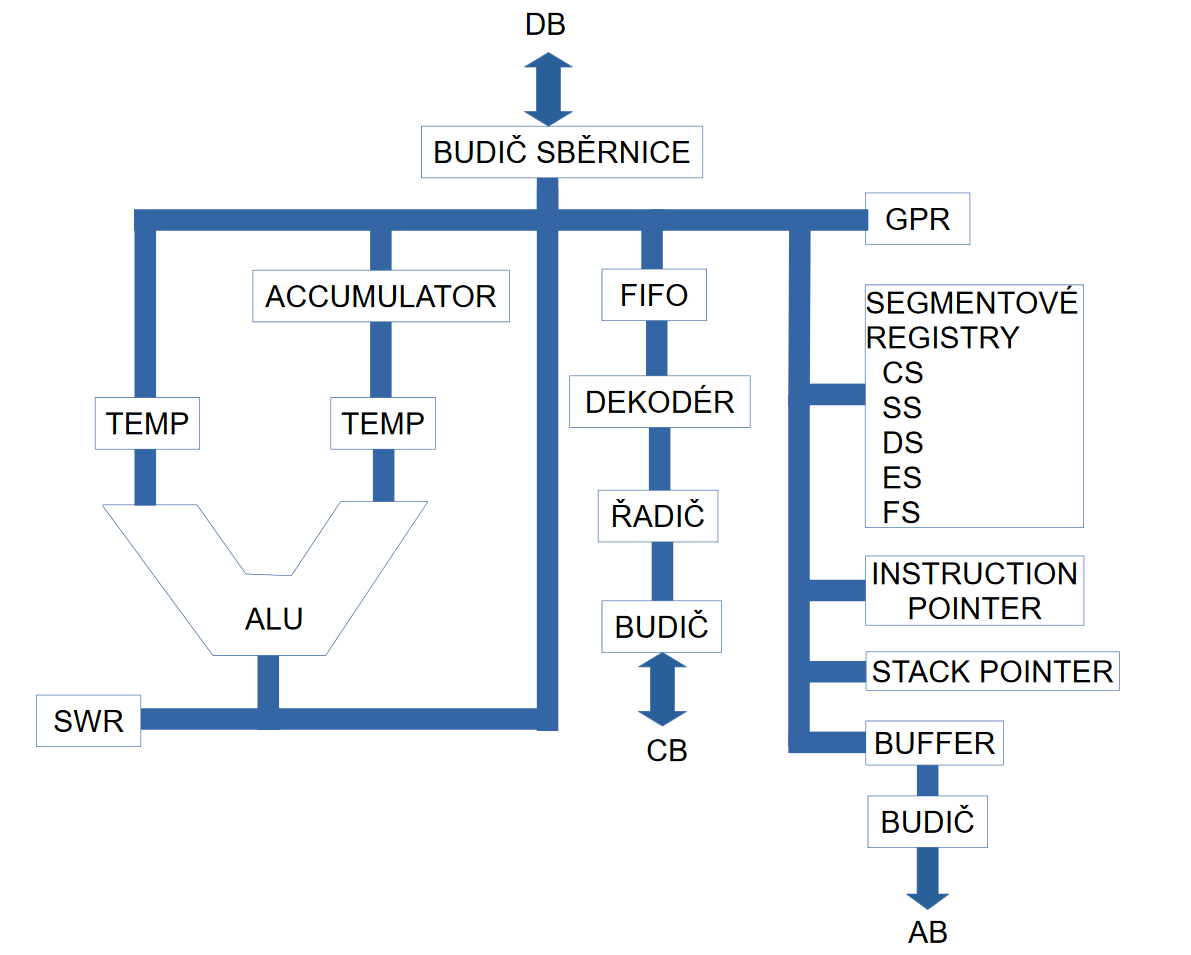
\includegraphics[width=15.778cm]{ref/blokove-schema-procesoru.png}
\item SWR -- registr stavového slova = stavy ALU
\item ALU -- provádí aritmetické a logické operace
\item TEMP -- je v něm vždy obsažen operand, zajišťuje konstantní vstupy
  během výpočtu
\item ACCUMULATOR

  \begin{itemize}
  \tightlist
  \item střádač -- většinou u menších procesorů
  \item slouží jako implicitní operand
  \item ukládá se do něj výsledek z ALU
  \item při instrukci ``přičti adresu'' - přičítá k ACC
  \end{itemize}
\item SBĚRNICE -- skupina vodičů se stejným protokolem
\item DB -- data bus -- datová sběrnice -- umožňuje výměnu dat
\item FIFO -- fronta instrukcí
\item DEKODÉR -- rozkládá instrukce na mikroinstrukce
\item ŘADIČ -- stará se o řídící sběrnice
\item GPR -- general purpose register -- víceúčelové registry
\item CS -- code segment
\item SS -- stack segment
\item CD -- data segment
\item ES -- extra segment
\item FS -- free segment
\item IP -- instruction pointer -- ukazatel instrukce, která se provede v
  následujícím kroku
\item SP -- stack pointer -- ukazatel zásobníku
\item AB -- address bus -- adresová sběrnice
\item výpočet adresy instrukce:

  \begin{itemize}
  \tightlist
  \item CS + IP =\textgreater{} adresa instrukce
  \item SS + SP =\textgreater{} adresa stacku
  \end{itemize}
\item jednodušší procesory mají ``program counter'' místo výpočtu adresy
  instrukce

  \begin{itemize}
  \tightlist
  \item obsahuje absolutní adresu
  \end{itemize}
\item provedení instrukce:

  \begin{itemize}
  \tightlist
  \item vezme se obsah těchto registrů (program counter nebo IP), najde se v
    paměti adresa a vezme se instrukce z buňky v paměti
  \item po provedení instrukce se zvedne IP nebo program counter a jednotku
    instrukce
  \end{itemize}
\item do stracku se zapisují adresy ze stack pointeru, které se neprovedly
  př.: kvůli přerušení
\item vždy se zapisuje na vrchol stacku
\item při zápisu se změnšuje pointer o jednotku instrukce
\item dno stacku se vytváří př.: zavedením programu do operační paměti
\item každý program má svůj stack
\item dno stacku je nejvyšší adresa
\item příklad:
\end{itemize}

\begin{minipage}[b]{0.75\textwidth}
    \begin{tabular}{|P{2cm}|P{2cm}|P{2cm}|P{2cm}|P{2cm}|}
        \hline
        kód instrukce & adresa prováděné instrukce & instruction pointer & stack pointer & obsah stacku \\ \hline
        & & A0 & D0 & AA \\ \hline
        MOV & A0 & A1 & D0 & AA \\
        INC & A1 & A2 & D0 & AA \\ \hline
        CALL B0 & A2 & A3 & D0 & AA \\
        & & A3 & CF & AB \\
        & & A3 & CF & A3 \\
        & & B0 & CF & A3 \\ \hline
        ADD & B0 & B1 & & \\
        MOV & B1 & B2 & & \\
        RET & B2 & B3 & & \\
        & & A3 & CF & A3 \\
        & & A3 & D0 & AA \\ \hline
        MOV & A3 & & & \\ \hline
    \end{tabular}
\end{minipage}%
\begin{minipage}[b]{0.25\textwidth}
    \begin{tabular}{|c|c|}
        \hline
        \multicolumn{2}{|P{3cm}|}{OPERAČNÍ PAMĚŤ} \\ \hline
        B3 & \\ \hline
        B2 & RET \\ \hline
        B1 & MOV \\ \hline
        B0 & ADD \\ \hline
        \multicolumn{2}{|l|}{} \\ \hline
        A5 & \\ \hline
        A4 & \\ \hline
        A3 & \\ \hline
        A2 & CALL B0 \\ \hline
        A1 & INC \\ \hline
        A0 & MOV \\ \hline
    \end{tabular}
\end{minipage}

\vspace{5mm}

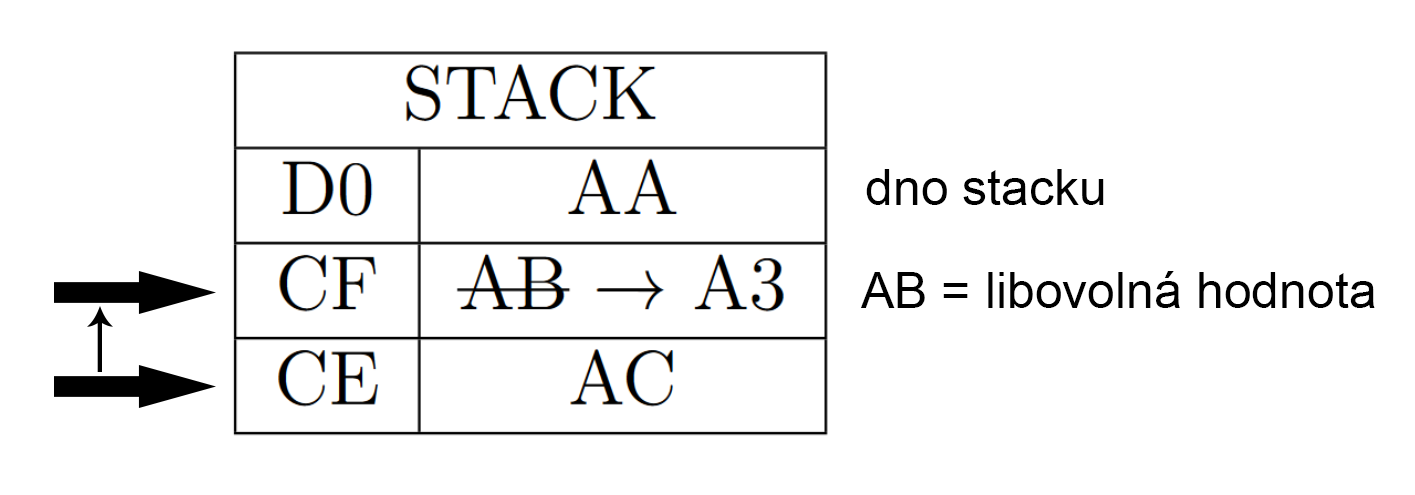
\includegraphics[width=8cm]{ref/podprogram-stack.png}

\begin{itemize}
\tightlist
\item aby mohl program začít, musí být první instrukce v IP nastavena na
  adresu z CB
\end{itemize}

\subsection{Přerušení}

\begin{itemize}
\tightlist
\item je to schopnost procesoru přerušit vykonávaný program a začít
  obsluhovat jiný
\item typy přerušení:

  \begin{itemize}
  \tightlist
  \item vnější -- asynchronní, neočekávané, neplánované -- přichází od
    vstupních zařízení
  \item vnitřní -- asynchronní, neočekávané, neplánované -- dělení nulou,
    výpadek zdrojů, procesoru chybí stránka
  \item softwarové -- synchronní, očekávané, plánované
  \end{itemize}
\item dělení přerušení:

  \begin{itemize}
  \tightlist
  \item maskovatelné -- není rozpoznat, že nastalo přerušení -- př.: ovladač
    něco potřebuje
  \item nemaskovatelné
  \end{itemize}
\item postup činnosti při přerušení:

  \begin{itemize}
  \tightlist
  \item signál přijímá řadič přerušení (interrupt controller)
  \item IC vyhodnocuje prioritu přerušení
  \item procesor dokončí právě prováděnou instrukci a následující instrukci
    uloží do stacku
  \item procesor si od řadiče vezme číslo přerušení
  \item procesoru v tabulce vektorů přerušení, hledá vektor přerušení --
    virtuální adresa první adresy přerušení
  \end{itemize}
\end{itemize}

\subsection{DMA}

\begin{itemize}
\tightlist
\item přímý přístup do paměti blokového zařízení bez použití procesoru

  \begin{itemize}
  \tightlist
  \item procesor naprogramuje DMA (probíhá v µs)
  \item DMA vyšle HOLD
  \item CPU potvrdí pomocí HOLD A (accepted)
  \end{itemize}
\item HP -- hardware procesor -- pracuje bez adresy
\item DMA řídí hardwarově -- jsou použity čítače
\end{itemize}

\subsection{RISC}

\begin{itemize}
\tightlist
\item má jednoduchý hardware
\item redukovaná instrukční sada

  \begin{itemize}
  \tightlist
  \item 2 instrukce pro práci s pamětí: LOAD, STORE
  \end{itemize}
\item program v assembleru bývá delší
\item co takt, to instrukce
\item je nutný pipelining
\item tento typ procesoru nemá pevný accumulator
\item dokáže přeadresovávat registry
\item je-li to výhodnější, umí přeorganizovat instrukce
\end{itemize}

\subsection{CISC}

\begin{itemize}
\tightlist
\item accumulator pevně vázaný na ALU
\item překlad instrukcí bývá dvojstupňový

  \begin{itemize}
  \tightlist
  \item rozloží se na mikroinstrukce -- ty se překládají do strojového kódu
  \end{itemize}
\item dnešní procesory se navenek jeví jako CISC, v jádře fungují jako
  RISCové procesory
\end{itemize}

\subsection{Parametry procesorů}

\begin{itemize}
\tightlist
\item frekvence je udávána v Hz, frekvence = počet instrukcí provedených za
  sekundu
\item efektivita mikrokódu -- počet kroků potřebných pro dokončení instrukce
\item numerický koprocesor -- FPU -- výpočty v pohyblivé čárce
\item počet instrukčních kanálů -- pipelining

  \begin{itemize}
  \tightlist
  \item počet instrukcí, které se zpracují v jednom taktu
  \end{itemize}
\item šířka slova -- maximální počet bitů, které je procesor schopen
  zpracovat během jedné operace
\item šířka přenosu dat -- počet bitů přenášených z procesoru nebo do
  procesoru
\item CACHE -- vyrovnávací paměť
\item velikost adresovatelné paměti
\item počet jader
\item chlazení -- aktivní, pasivní, kombinované

  \begin{itemize}
  \tightlist
  \item pasivní -- žebrovaný chladič vyrobený z materiálu, který velmi dobře
    odvádí teplo
  \item aktivní -- větráček
  \item kombinovaný -- nejčastější
  \item vodní chlazení
  \end{itemize}
\end{itemize}

\subsubsection{Pipelining}

\begin{itemize}
\tightlist
\item zřetězené zpracování instrukcí
\item nejčastěji pětistupňový
\item procesor je rozdělen na subprocesory

  \begin{itemize}
  \tightlist
  \item ve stejném okamžiku pracují na jiných instrukcích jiní části
    procesoru
  \item výsledek ukládají do společné paměti
  \end{itemize}
\item rozdělení na kroky:

\begin{enumerate}
    \def\labelenumii{\arabic{enumii}.}
    \tightlist
    \item čtení
    \item dekódování
    \item provedení
    \item zapsání do paměti
    \item zaznamenání do registru
\end{enumerate}
\end{itemize}

\begin{tabular}{|P{2cm}|c|c|c|c|c|}
\hline
čas okamžiku / subproces & 1 & 2 & 3 & 4 & 5 \\ \hline
1 & A & & & & \\ \hline
2 & B & A & & & \\ \hline
3 & C & B & A & & \\ \hline
4 & D & C & B & A & \\ \hline
5 & E & D & C & B & A \\ \hline
\end{tabular}

\subsubsection{Super skalární procesor}

\begin{itemize}
\tightlist
\item jeden ze způsobů jak zvýšit výkon procesoru, př.: více ALU, FPU
\item navenek se jeví jako jeden procesor
\item v jednom taktu zpracuje více informací následujících za sebou
\end{itemize}

\subsubsection{Vícejádrové procesory}

\begin{itemize}
\tightlist
\item jádro obsahuje ALU, řadič, registry
\item nepoužitá jádra se vypnou pro šetření energie
\item každý proces je tvořen vlákny

  \begin{itemize}
  \tightlist
  \item proces je někdy nazýván odlehčený proces)
  \end{itemize}
\item OS musí podporovat vlákna
\item procesy mají oddělený adresový prostor
\item vlákna mají společný adresový prostor
\item jádra mají svoji cache a mají také společnou cache
\item jádra a cache jsou prpojené crossbarovými sběrnicemi
\item každé jádro má řadič přerušení a řídí si přerušení
\item volné jádro může obsloužit přerušení zaneprázdněného jádra
\end{itemize}

\subsubsection{Hyperthreading}

\begin{itemize}
\tightlist
\item jeden fyzický procesor se navenek jeví jako dva logické procesory
\item jsou duplikovány regisry a řadič přerušení
\item procesor na vstupu přijme dvě vlákna za předpokladu, že každé vlákno
  potřebuje jinou výkonnou jednotku, v jiném případě jedno vlákno čeká
  na zpracování
\item technologie používaná Intelem
\end{itemize}

\subsubsection{HyperTransport}

\begin{itemize}
\tightlist
\item obousměrná (full duplex)
\item umožňuje vysokou propustnost
\item propojuje procesor k severnímu mostu
\end{itemize}

\subsubsection{Multithreading}

\begin{itemize}
\tightlist
\item současně se bude zpracovávat více vláken
\end{itemize}

\subsubsection{Multiprocesor}

\begin{itemize}
\tightlist
\item centrálně řízený systém s více procesory se společnou pamětí
\item procesory jsou soustředěny kolem jedné sběrnice
\item vhodné pro řešení jedné úlohy
\item řízení zařizuje jeden operační systém
\item používá se tam kde je potřeba vysoké spolehlivosti systému
\end{itemize}

\subsubsection{Procesorová pole}

\begin{itemize}
\tightlist
\item vytvořeno ze stejných procesorů navzájem propojených
\item mají centrální řadič
\item každý procesor má vlastní paměť
\item data se dají přesouvat mezi sousedními procesory
\item vstupní data se dávají do krajních procesorů, které jsou přímo
  napojeny na sběrnici
\item liší se od paralelního zapojení (multiprocesory) tím, že každý
  procesor má svoji paměť
\item[] 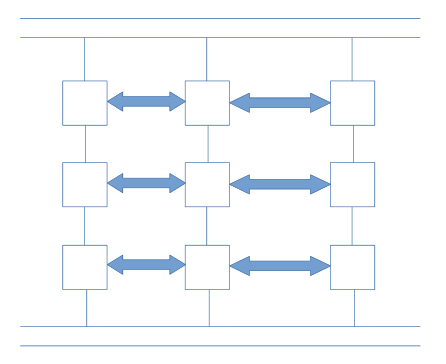
\includegraphics[width=6.034cm]{ref/paralelni-procesory.png}
\end{itemize}

\section{Periferie, klávesnice, myš}

\subsection{Klávesnice}

\begin{itemize}
\tightlist
\item kontaktní, bezkontaktní klávesy
\item klávesnice rozvržena do matice
\item mechanické, membránové (halové a kapacitní)
\item fungování klávesnice -- SCAN kódy

  \begin{itemize}
  \tightlist
  \item po stisku je vygenerován SCAN kód, ten jde přes buffer klávesnice na
    řadič na základní desce, tam mu je přiřazena stisknutá klávesa podle
    SCAN kódu
  \end{itemize}
\end{itemize}

\subsection{Kuličková myš}

\begin{itemize}
\tightlist
\item 2 snímače navzájem posunuty o $\frac{\pi}{2}$ = 90°
\item na hřídelce je clonkové kolečko
\item světelný paprsek dopadá na senzor podle toho zda prosvítá
\end{itemize}

\subsection{DSP -- Digital Signal
Processor}

\begin{itemize}
\tightlist
\item používá se u optických myší
\item snímky z povrchu se ukládají v CMOS myši a podle rozdílů v obrazech se
  vypočítá směr a vzdálenost pohybu
\end{itemize}

\subsection{Joystick}

\begin{itemize}
\tightlist
\item pákový ovladač
\item digitální nebo analogový
\item použití: hry, průmyslová zařízení, letadla
\item dříve se připojoval přes gameport, nyní USB
\item má dvě osy -- \emph{x}, \emph{y} (případně i osu \emph{z} pro
  naklánění)
\end{itemize}

\section{Virtualizace RAM v PC, stránkování, swapování, výpočet adres v protected módu}

\begin{itemize}
\tightlist
\item každý počítač startuje v real módu
\item real mód má velikost paměti do 1MB
\item adresová sběrnice má 20 bitů
\item registry jsou 16 bitové
\item segment + offset = fyzická adresa
\item CS + IP = fyzická adresa
\item CS * 16 + IP = fyzická adresa instrukce v real módu
\item př.: segment 020A; offset 1BCD

  \begin{itemize}
  \tightlist
    \item[] $\frac{{{020A} \atop {1BCD}}}{1DD7}$
  \end{itemize}
\end{itemize}

\subsection{Výpočet adresy v protected módu}

\begin{itemize}
\tightlist
\item protected mód = chráněný režem -- chrání pamět programů proti zápisu z
  jiných programů
\item zapisuje do paměti nad 1~MB
\item[] 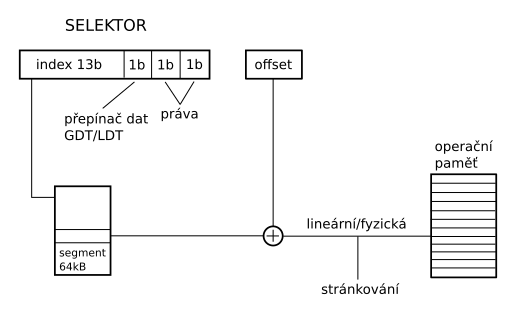
\includegraphics[width=13.651cm]{ref/vypocet-logicke-adresy.png}
\item logická adresa = selector + offset
\item \emph{index} ukazuje na řádek tabulky, ten má 8~B, skládá se z:
\end{itemize}

\begin{tabular}{|c|c|c|}
\hline
& 32~bit & 16~bit \\ \hline
báze & 4~B & 3~B \\ \hline
limit & 3~B & 2~B \\ \hline
práva + atributy & 1~B & 1~B \\ \hline
rezerva & & 2~B \\ \hline
\end{tabular}

\begin{itemize}
\tightlist
\item báze -- počáteční adresa segmentu
\item limit -- velikost segmentu, musí být menší než offset
\item práva -- archivní, systémové, obyčejný uživatel
\item rezerva -- pro \emph{bázi} a \emph{limit}
\end{itemize}

\subsection{GDT/LDT}

\begin{itemize}
\tightlist
\item global descriptor table

  \begin{itemize}
  \tightlist
  \item jediná pro operační systém, její adresa se přepne do real módu
  \end{itemize}
\item local descriptor table

  \begin{itemize}
  \tightlist
  \item adresy jsou v GDT
  \end{itemize}
\item tabulky deskriptorů (popisovačů)

  \begin{itemize}
  \tightlist
  \item popisují systém uložení
  \end{itemize}
\item segment = tabulka
\item každý segment má 8 řádků (celkem 64~kB)
\item práva -- archivní, systémové, obyčejný uživatel
\end{itemize}

\subsection{Stránkování}

\begin{itemize}
\tightlist
\item rozdělení paměti na úseky konstantní velikosti
\item základní velikost: 4~kB
\item velikost záleží na operačním systému -- stanoví se při zavedení
  systému
\item[] 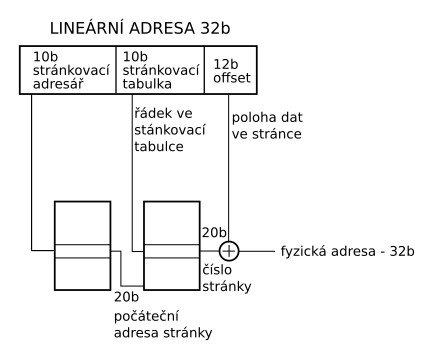
\includegraphics[width=11.455cm]{ref/strankovani-fyzicka-adresa.png}
\item výhody stránkování
  \begin{itemize}
    \tightlist
    \item nejsou potřeba kontroly (díky konstantní velikosti)
    \item rychlé zpracování
  \end{itemize}
\end{itemize}

\subsection{Virtuální paměť (swapování)}

\begin{itemize}
\tightlist
\item operační paměť je někdy příliš malá pro programy, proto se rozšiřuje o
  virtuální paměť
\item ukládají se zde momentálně nepotřebné stránky
\item uplatňuje se při swapování
\item swapovací prostor rozšiřuje operační paměť
\item různé OS řeší různými způsoby
\item swapuje se po stránkách

  \begin{itemize}
  \tightlist
  \item stránku ve swapovacím prostoru nazýváme frame
  \end{itemize}
\item MMU -- memory management unit

  \begin{itemize}
  \tightlist
  \item najde v operační paměti stránky, které nebudou potřeba, najde volný
    frame a zapíše je na disk
  \item číslo framu se přepíše číslem stránky a přidá se flag o tom kde se
    nachází (swap nebo RAM)
  \end{itemize}
\item swapování je odkládání momentálně nepotřebných dat do virtuální paměti
  a vracení dat do operační paměti v momentě kdy jsou data potřeba
\item swapovací prostor by měl být dvojnásobně větší jak operační paměť
\item při swapování nastává zpoždění, proces swapování je velmi pomalý
\end{itemize}

\section{24. Zásobníkové procesory, módy procesorů}

\subsection{Zásobníkové procesory}

\begin{itemize}
\tightlist
\item používají se tam, kde se používají řídící systémy
\item jsou založeny na základě 2 zásobníků

  \begin{itemize}
  \tightlist
  \item zásobník operandů
  \item zásobník návratových adres
  \end{itemize}
\item zásobník je na principu LIFO
\item jsou jednodušší než procesory CISC a RISC
\item mají kratší instrukční sadu
\item mají dvou stupňový pipelining
\item chybí fáze dekódování
\item operandy jsou v prvních 2 položkách zásobníku
\item ALU má v každý okamžik operandy ke zpracování
\item zásobníkové procesory nezahazují instrukce
\item na přerušení reagují se zpožděním pouze 1 strojového cyklu
\item ALU má šířku operandů 20 bitů
\item jedno instrukční slovo: max 4 instrukce
\item šířka jedné instrukce je 5 bitů
\item nemá cache
\item počet instrukcí: $2^{32}$
\end{itemize}

\subsection{Módy 64 bitových procesorů}

\begin{itemize}
\tightlist
\item[] 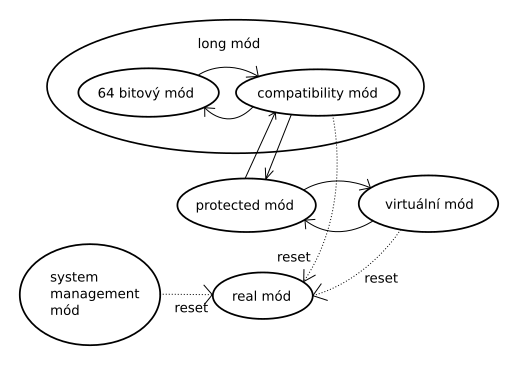
\includegraphics[width=13.704cm]{ref/mody.png}
\item long, legacy
\item existuje přepínání mezi módy
\item počítač startuje v \emph{reálném režimu}
\item \emph{virtuální mód} se dnes nepoužívá

  \begin{itemize}
  \tightlist
  \item umožňuje spouštět programy určeny pro reálný režim s výhodami
    chráněného režimu
  \end{itemize}
\item system management mód

  \begin{itemize}
  \tightlist
  \item extra povolení
  \item je určen pro řízení systémových aktivit (systémový mód)
  \item někdy se nazývá nastavovací mód
  \end{itemize}
\item long mód umožňuje používat 64 bitový mód nebo compatibility mód

  \begin{itemize}
    \tightlist
  \item 64 bit mód

    \begin{itemize}
    \tightlist
    \item je určený pro 64 bitové procesory
    \item má 64 bitové registry a instruction pointer
    \item flat segmentustránkování
    \end{itemize}
  \item režim kompatibility

    \begin{itemize}
    \tightlist
    \item je kompatibilní s 16 bit a 32 bit procesory -- je možné spouštěť
      programy navržené pro tyto procesory
    \item neobsazené bity jsou vyplněny 1 případně 0
    \end{itemize}
  \end{itemize}
\item legacy mód

  \begin{itemize}
  \tightlist
  \item nemají všechny procesory (AMD ano, Intel ne)
  \item pracuje jako opravdový 32 bitový procesor (s kompatibilitou pro 16
    bit procesory)
  \item registry nepřetěžuje zbytečnými bity doplňující do 64~b
  \end{itemize}
\end{itemize}

\subsection{Adresování}

\begin{itemize}
\tightlist
\item long mód inplementuje ``flat model''
\item flat model představuje jeden segment (původně přes celou paměť)
\item u 32~bit do 1~MB
\item rozeznáváme 4 druhy adres

  \begin{itemize}
    \tightlist
  \item \emph{logická} -- báze, vstupní adresa pro výpočet
  \item \emph{efektivní adresa} -- offset
  \item \emph{lineární adresa} = báze + offset
  \item u flat modelu je počáteční adresa segmentu rovna 0 tzn. že lineární
    adresa je shodná s efektivní adresou proto se udává v kanonickém
    tvaru
  \item kanonická forma adresy

    \begin{itemize}
    \tightlist
    \item vyžaduje, aby všechny bity 48--46 opakovaly 47-mý bit
    \end{itemize}
  \item fyzická adresa -- určuje polohu ve fyzickém prostoru
  \item[] 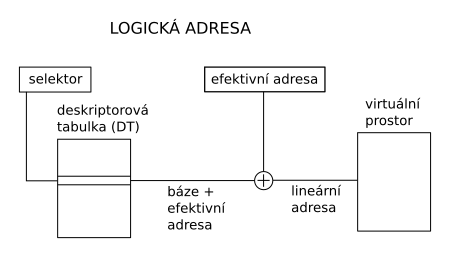
\includegraphics[width=11.904cm]{ref/logicka-adresa.png}
  \end{itemize}
\end{itemize}

\subsection{Stránkování}

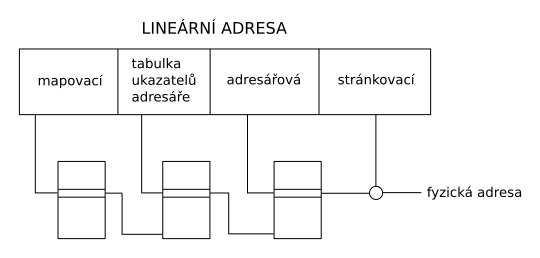
\includegraphics[width=12cm]{ref/strankovani.png}

\section{Paměti}

\subsection{Paměti podle fyzikálního rozdělení}

\subsubsection{Polovodičové}

\begin{itemize}
\tightlist
\item statické
\item dynamické
\item PROM, EPROM, EEPROM
\end{itemize}

\subsubsection{S pohyblivou magnetickou vrstvou}

\begin{itemize}
\tightlist
\item magnetické disky
\item diskety
\item kazety
\end{itemize}

\subsubsection{Optické}

\begin{itemize}
\tightlist
\item DVD, CD, Blu-Ray
\end{itemize}

\subsubsection{Magnetooptické}

\subsection{Podle závislosti na napájení}

\subsubsection{Závislé (volatilní)}

\begin{itemize}
\tightlist
\item uchování a přístup k datům je závislý na napájení
\item př.: polovodičové paměti
\end{itemize}

\subsubsection{Nezávislé (nevolatilní)}

\begin{itemize}
\tightlist
\item nepotřebují k uchování dat napájení, pouze k přístupu
\end{itemize}

\subsection{Podle přístupu do paměti}

\subsubsection{RAM}

\begin{itemize}
\tightlist
\item paměti s náhodným přístupem
\item přístup není závislý na adrese umístění
\item polovodičová paměť
\end{itemize}

\subsection{Podle schopnosti zápisu}

\begin{itemize}
\tightlist
\item pro čtení a zápis
\item ROM -- pouze pro čtení

  \begin{itemize}
  \tightlist
  \item zápis se provede při výrobním procesu a je neměnný
  \end{itemize}
\item write-only memory -- př.: černá skříňka
\end{itemize}

\subsection{Vnitřní paměti}

\begin{itemize}
\tightlist
\item k práci potřebují procesor
\item cache, registry, CMOS
\end{itemize}

\subsection{Vnější paměti}

\begin{itemize}
\tightlist
\item slouží k trvalému uchování dat
\item HDD, CD, DVD, diskety, kazety, paměťové karty
\end{itemize}

\subsection{Destruktivnost při čtení}

\begin{itemize}
\tightlist
\item u destruktivních pamětí se informace po přečtení zmizí a je potřeba ji
  znovu zapsat
\item u nedestruktivních pamětí zůstávají data po přečtení bez změny
\item polovodičová paměť se skládá z buněk
\item paměťová banka je zastávána integrovaným obvodem
\item každá buňka může mít hodnotu 1 nebo 0
\item paměťové buňky jsou uspořádány do matice (tvoří mřížku)
\item poloha buňky je určena řádkovým a sloupcovým vodičem
\item paměťový řadič řídí čtení a zápis

  \begin{itemize}
  \tightlist
  \item bipolární tranzistory
  \item[] 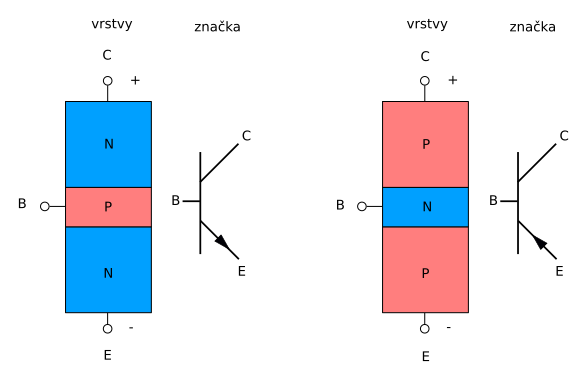
\includegraphics[width=15.529cm]{ref/bipolarni-transistory.png}
  \item unipolární tranzistory
  \item[] 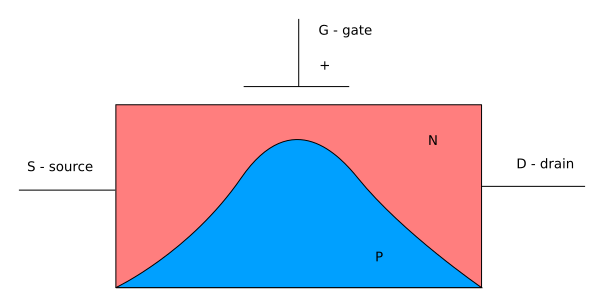
\includegraphics[width=15.73cm]{ref/unipolarni-tranzistor.png}
  \end{itemize}
\end{itemize}

\subsection{Volatilní}

\subsubsection{Statické paměti}

\begin{itemize}
\tightlist
\item uchovávají informace po celou dobu kdy jsou připojeny k napájení
\item přístupová doba 1~ns -- 20~ns
\item složitější, vyšší výrobní náklady než dynamické paměti
\item je rychlejší
\item je tvořena bistabilním klopným obvodem
\item používá se na výrobu CMOS, cache (L1, L2, L3)
\end{itemize}

\subsubsection{Dynamické paměti}

\begin{itemize}
\tightlist
\item informace je uložena jako elektrický náboj na kondenzátoru
\item náboj se vybíjí i při připojeném napájení -- je nutný refresh
\item v době refreshe není možné číst ani zapisovat
\item buňka má jednoduchou výrobu, nízké náklady na výrobu
\item přístupová doba 10~ns -- 70~ns
\item čtení je destruktivní -- informace musí být znovu zapsána po přečtení
\end{itemize}

\subsection{Nevolatilní}

\begin{itemize}
\tightlist
\item často se používají pro firmware
\end{itemize}

\subsubsection{ROM}

\begin{itemize}
\tightlist
\item informace je zapsána při výrobě a nelze změnit
\item př.: firmware
\end{itemize}

\subsubsection{PROM}

\begin{itemize}
\tightlist
\item programmable read only memory
\item vyrobí se bez informace -- uživatel může zapsat informaci, poté ji
  nelze měnit
\end{itemize}

\subsubsection{EPROM}

\begin{itemize}
\tightlist
\item je možné ji vymazat UV zářením
\end{itemize}

\subsubsection{EEPROM}

\begin{itemize}
\tightlist
\item mazání se provádí pomocí elektrického impulzu
\end{itemize}

\subsection{Flash ROM}

\begin{itemize}
\tightlist
\item elektricky programovatelná paměť
\item paměť je organizována po blocích
\item př.: firmware, vnější medium
\item data bez napětí vydrží uchována \textasciitilde{}10 let
\end{itemize}

\subsection{Dynamická paměť}

\subsubsection{Blokové schéma dynamické paměti}

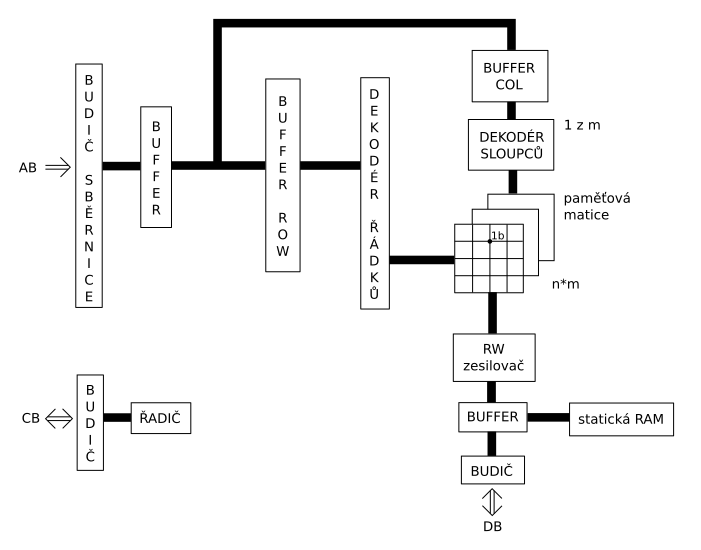
\includegraphics[width=17cm]{ref/blokove-schema-dynamicke-pameti.png}

\begin{itemize}
\tightlist
\item řadič je propojen se vším
\item když je adresa v bufferu, je možné načíst další adresu
\item paměťových matic je několik

  \begin{itemize}
  \tightlist
  \item jsou společně ovládány
  \item mají každá svůj vstup a výstup
  \item šířka datové sběrnice = počet matic
  \end{itemize}
\item RW zesilovač -- dělá z elektrického signálu logický signál
\item paměť je destruktivní, proto je zde statická RAM -- do té se informace
  při čtení uloží a následně se znovu zapíše
\end{itemize}

\subsubsection{Časový diagram paměti}

\begin{itemize}
\tightlist
\item[] 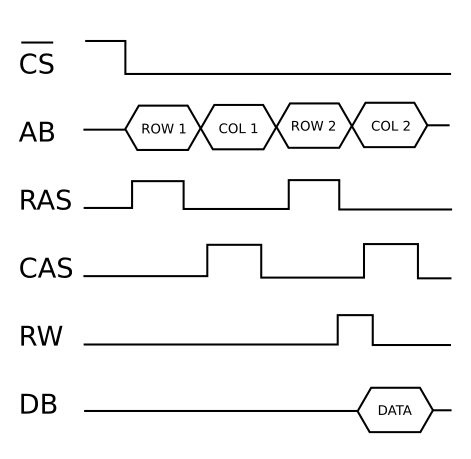
\includegraphics[width=12.46cm]{ref/casovy-diagram-dynamicke-pameti.png}
\item časování v nanosekundách 5 - 2 - 2 - 2
\end{itemize}

\subsubsection{Synchronní paměť EDO}

\begin{itemize}
\tightlist
\item datová sběrnice je obsazená pouze kdy se čtou nebo zapisují data
\end{itemize}

u asynchronní je datová sběrnice obsazena vždy

\begin{itemize}
\tightlist
\item CS -- chip select -- výběr obvodu, který bude reagovat

  \begin{itemize}
  \tightlist
  \item negovaný z bezpečnosti, aby při přerušení vše zůstalo nefunkční
  \end{itemize}
\item AB -- adresový sběrnice
\item RAS -- row address or strobe -- říká, že signál na sběrnici je platný
\item CAS - column address or strobe
\item RW -- log. 1 říká, že data jsou platná + signál pro čtení, zápis
\item paměť může být typu \emph{burst}

  \begin{itemize}
  \tightlist
  \item může pracovat s více adresami -- ukládají se do mini cache
  \item při opětovném čtení je již uloženo v mini cache -- tím se paměť
    zrychluje
  \end{itemize}
\end{itemize}

\subsection{Magnetické paměti}

\begin{itemize}
\tightlist
\item v závislosti na změně proudu se mění magnetická indukce
\item když se zmenšuje \emph{H} -- intenzita magnetického pole, zmenšuje se
  i magnetická indukce

  \begin{itemize}
    \tightlist
  \item ne však do nuly, zastaví se na \emph{Br} -- magnetická remanence --
    zbytek magnetismu, který si materiál uchovává po konci působení
    magnetického pole
  \item v \emph{Br} se změní směr proudu → \emph{H} se nebude zvětšovat →
    max \emph{Hc}
  \item Hc -- koercitivita (koercivita) udává magnetickou tvrdost

    \begin{itemize}
    \tightlist
    \item hodnota nutná k odmagnetování materiálu
    \item když budu dál zvětšovat → dojde k nasycení v opačném směru
    \end{itemize}
  \end{itemize}
\end{itemize}

\subsubsection{Hard disk}

\begin{itemize}
\tightlist
\item vnější paměť
\item slouží k trvalému uchování dat
\item velkokapacitní
\item pohyblivá magnetická vrstva
\item energeticky nezávislý (nevolatilní)
\item HDD se skládá z ploten a hlav
\item plotna může být kovová nebo skleněná, pevná a neohebná
\item je pokryta tenkou vrstvou magneticky citlivého materiálu
\item na magnetické vrstvě je vrstva maziva -- chrání proti mechanickému
  poškození
\item průměr plotny 3.5" nebo 2.5"
\item ploten může být více nad sebou
\item hlava zajišťuje čtení a zápis
\item hlava pluje na vzduchovém polštáři nad plotnou
\item na každou plotnu jsou dvě hlavy -- z obou stran jedna
\item vystavovací mechanismus -- vystaví hlavu na správnou pozici

  \begin{itemize}
  \tightlist
  \item 3 fáze: seek time, settle time, latence
  \item seek time -- nalezení pozice na disku, vystřelení hlavy
  \item settle time -- čekání na utlumení kmitání hlavy (v ms)
  \item latence -- vyčká se na pootočení disku
  \end{itemize}
\item čím rychleji se disk točí, tím je latence nižší
\item při čtení a zápisu prochází hlavou proud, který zmagnetizuje vrstvu
\item každý disk obsahuje řadič -- řídí čtení a zápis

  \begin{itemize}
  \tightlist
  \item obsahuje paměť typu ROM -- obsahuje firmware
  \item řídí pohon, dekódování, kódování
  \end{itemize}
\item konfigurační přepínače -- jumpery
\item kontroluje rychlost otáčení
\item CACHE -- k uložení dat před zápisem; když jsou data v CACHE, tak disk
  hlásí, že data zapsal
\item motor -- zajišťuje otáčení ploten; pouzdro motoru je z nemagnetického
  materiálu
\item rychlost otáčení ploten:

  \begin{itemize}
  \tightlist
  \item u notebookových HDD: 4200 ot./min. - menší spotřeba energie
  \item u standardních disků: 7200 ot./min.
  \item u lepších disků: 10000 ot./min.
  \end{itemize}
\item disk musí být hermeticky uzavřený
\item disky jsou náchylné na mechanické rázy
\item hlavy jsou zaparkovány mimo datovou plochu, když je disk vypnutý
\item rozhraní:

  \begin{itemize}
    \tightlist
  \item ATA = IDE = PATA = ATAPI

    \begin{itemize}
    \tightlist
    \item 40 pinový konektor
    \item paralelní rozhraní
    \item master a slave
    \end{itemize}
  \item SATA -- úzký kabel, sériový, podporuje Hot swap
  \item SCSI

    \begin{itemize}
    \tightlist
    \item výkonné pracovní stanice, servery
    \item 68 pinový konektor
    \item lze připojit různé periferie
    \end{itemize}
  \item USB, Firewire

    \begin{itemize}
    \tightlist
    \item externí disky
    \end{itemize}
  \end{itemize}
\item bity jsou uloženy horizontálně na ploše disku -- menší hustota zápisu
\item kolmý záznam -- umožňuje zvýšení hustoty záznamu

  \begin{itemize}
  \tightlist
  \item asymetrický magnet, stabilizační vrstva
  \item tenký pól se stará o to aby magnetické pole směřovalo co nejvíce do
    hloubky
  \item široký nástavec má malou hustotu siločar
  \item tenký pól soustředí siločáry do úzkého prostoru umožňující
    magnetizaci
  \item každý bit vytváří miniaturní dipól
  \item siločáry musí procházet přes stabilizační vrstvu
  \end{itemize}
\end{itemize}

\paragraph{Geometrie pevného disku}

\begin{itemize}
\tightlist
\item[] 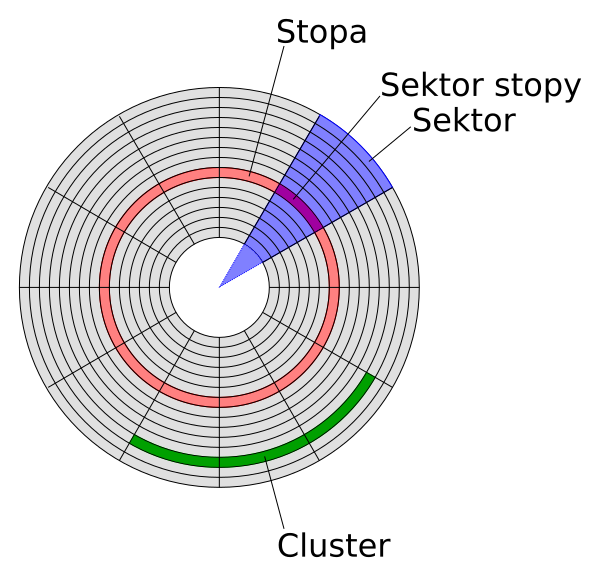
\includegraphics[width=10.089cm]{ref/geometrie-disku.png}
\item popisuje počet stop, sektorů, cylindrů, clusterů, počet hlaviček
\item Low Level Format -- nízkoúrovňový; je prováděn výrobcem disku
\item sektor -- nejmenší možná adresovatelná jednotka disku -- původně 512
  B, dnes 4 kB
\item cylindr -- sada stop se stejným číslem na různých stranách ploten
\item cluster -- alokační jednotka tvořena operačním systémem -- je nejmenší
  použitelná šířka data pohromadě
\item velikost clusteru je dána použitým souborovým systémem
\item cluster je obsazen i když není zcela plný
\end{itemize}

\paragraph{Prokládání}

\begin{itemize}
\tightlist
\item je jednou z metod, která zkracuje dobu čekání
\item bez prokládání se při čtení se provedou data z 1. sektoru, pošlou se
  přes řadič aplikaci a je dotaz na další data, pro čtení se musí počkat
  celou otáčku disku
\end{itemize}

\subparagraph{ZBR}

\begin{itemize}
\tightlist
\item Zone bit recording
\item zvyšuje kapacitu disku
\item stopy u středu jsou kratší a mají tím méně sektorů, proto se na vnější
  stopy dá více sektorů
\end{itemize}

\paragraph{Kapacita disku}

\begin{itemize}
\tightlist
\item vypočte se jako \emph{cylindr * hlava * sektor}
\end{itemize}

\paragraph{Metody adresace}

\begin{itemize}
\tightlist
\item CHS = cylindr × hlavičky × sektory

  \begin{itemize}
  \tightlist
  \item nepoužívá se, je zastaralá
  \end{itemize}
\item $LBA = (C \times HPC + H) \times SPT + (S - 1)$

  \begin{itemize}
  \tightlist
  \item logical block addressing
  \item C -- cylindr
  \item HPC -- max počet hlav na cylindr
  \item SPT -- max počet sektorů na pevném disku
  \item S -- stopa
  \item tato metoda očísluje všechny sektory na pevném disku
  \item z daného čísla je pak každému přidělena nová 8 bitová adresa
  \item jelikož se podle tohoto vztahu vypočte vlastní číslo, není nutné
    znát geometrii disku
  \end{itemize}
\end{itemize}

\paragraph{Parametry HDD}

\begin{itemize}
\tightlist
\item formát: 3.5", 2.5"
\item rozhraní: ATA, SATA
\item kapacita: v GB, TB
\item otáčky: 5400 RPM, 7200 RPM, 10000 RPM

  \begin{itemize}
  \tightlist
  \item více otáček → více tepla → je potřeba lepší chlazení
  \end{itemize}
\item vyrovnávací paměť 2 MB, 16 MB
\item přístupová doba: průměrná doba za kterou je disk připraven číst nebo
  zapsat (v ms)
\item celkový výkon: podle rychlosti
\item hlučnost
\item spotřeba energie
\item přenosová rychlost
\item odolnost vůči otřesům
\item hmotnost
\end{itemize}

\paragraph{S.M.A.R.T.}

\begin{itemize}
\tightlist
\item Self-Monitoring, Analysis and Reporting Technology
\item provádí monitorování, analyzování a hlášení chyb
\item zprávy se posílají operačnímu systému
\item chyby: předvídatelné a nepředvídatelné
\item S.M.A.R.T. analyzuje pouze předvídatelné chyby:

  \begin{itemize}
  \tightlist
  \item poškození povrchu
  \item poškození hlavy: měkké chyby -- opakované čtení
  \item poškození motoru: narůstá čas k roztočení disku
  \item hlava se vychyluje, není schopno sledovat stopu
  \item poškození vystavovacího mechanismu
  \end{itemize}
\item nepředvídatelné chyby:

  \begin{itemize}
  \tightlist
  \item poškození disku náhlým přepětím
  \item poškození špatným zacházením
  \item poškození nadměrným teplem, magnetickým polem
  \end{itemize}
\end{itemize}

\paragraph{Cachované disky}

\begin{itemize}
\tightlist
\item všechny dnešní disky jsou cachované
\item dochází k vyrovnání rychlosti dat
\item cache je statická paměť
\item zaručuje konstantní rychlost mezi operační pamětí nebo DMA
\item v disku je řadič, který řídí cache
\end{itemize}

\paragraph{Disková pole}

\begin{itemize}
\tightlist
\item soustavy pevných disků
\item informace se paralelně zapisuje do několika disků zároveň, tím je
  dosažena vyšší spolehlivost
\item \textbf{RAID} -- redundant array of independent disks -- vícenásobné
  pole nezávislých disků
\item RAID 0

  \begin{itemize}
  \tightlist
  \item systém postupného čtení a zápisu na více disků
  \item v jednom okamžiku systém pracuje s jedním diskem a při zaplnění
    stopy se přepne na druhý disk; první si bude mezitím nastavovat
    stopu
  \item je bez zálohování
  \item při poruše jednoho z disků se systém zhroutí
  \end{itemize}
\item RAID 1

  \begin{itemize}
  \tightlist
  \item mirroring -- zrcadlení
  \item zapisuje se na disky zároveň
  \item čte se z disku který je blíž datům
  \end{itemize}
\item RAID 5

  \begin{itemize}
  \tightlist
  \item paritní informace se ukládají na všechny disky
  \item minimum disků jsou 3 disky
  \end{itemize}
\item RAID 6

  \begin{itemize}
  \tightlist
  \item obsahuje 2 paritní disky
  \item mohou vypadnout 2 disky
  \item pomalejší zápis
  \end{itemize}
\item RAID 7

  \begin{itemize}
  \tightlist
  \item má navíc centrální cache
  \end{itemize}
\item RAID 10

  \begin{itemize}
  \tightlist
  \item spojení RAID 0 a RAID 1
  \item data se nejdříve zrcadlí a potom se uloží do pole RAID 0
  \item použití pro databázové systémy
  \end{itemize}
\end{itemize}

\subsection{Optické disky}

\begin{itemize}
\tightlist
\item průměr 12 cm
\item zaznamená se na něj 84 minut -- 750 MB
\item malé disky o průměru 8 cm -- až 24 minut -- 210 MB
\item stejně velké sektory
\item princip čtecí a optické hlavy:
\item[] 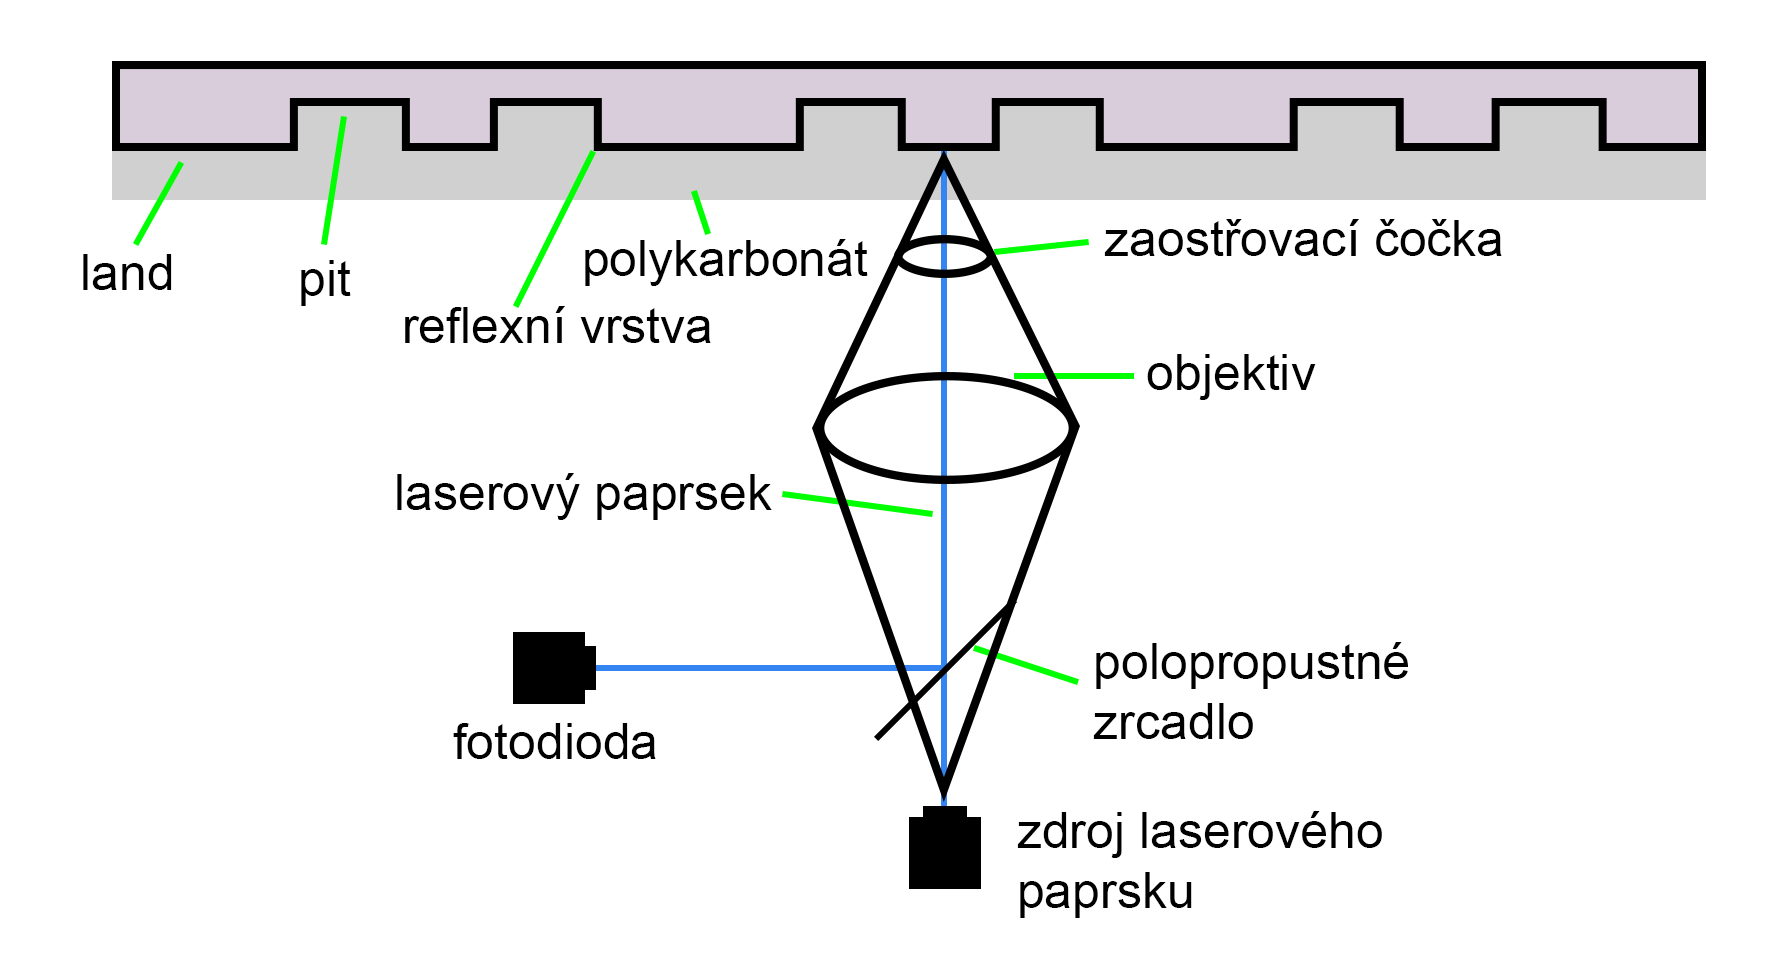
\includegraphics[width=12.896cm]{ref/princip-cteci-a-opticke-hlavy.png}
\item fotodioda -- převádí světelný impuls na elektrický
\item data jsou poslána na DAC -- digitálně analogový převodník; převádí
  digitální signál na analogový
\item LAND -- plocha disku
\item PIT -- díra; v pitu se světlo rozptýlí → žádný odraz → žádné napětí
\item přechod mezi pitem a landem je logická 1
\item žádná změna je logická 0
\item informaci nese každá změna z 1 na 0 a z 0 na 1
\end{itemize}

\end{document}
